\subsection{Xarxa neuronal amb una capa oculta}

En aquesta secció s'explicarà el desenvolupament del mètode de xarxes neuronals, en concret s'usarà el mètode de perceptró multicapa amb una capa oculta.

Primer de tot es necessita determinar el nombre de neurones que disposarà la capa oculta. Sabem que la capa d'entrada tindrà 16 neurones, una per cada característica, i la capa de sortida 26 neurones, una per cada classe. Per la capa oculta usarem \textit{5-fold Cross-Validation} per tal de determinar el nombre de neurones a usar. De la mateixa manera, per tal d'evitar el sobreajust en el conjunt de dades d'entrenament i que el nostre model pugui generalitzar millor, usarem regularització. Per tant, en realitzar \textit{Cross-Validation} trobarem la millor combinació de neurones juntament amb el seu valor de regularització.

\begin{table}[ht]
\centering
\begin{adjustbox}{max width=\textwidth}
\begin{tabular}{|r|r|r|r|r|r|}
  \hline
size & decay & Accuracy & Kappa & AccuracySD & KappaSD \\ 
  \hline
  28 & 0.50 & 0.8895 & 0.8851 & 0.0044 & 0.0046 \\ 
  28 & 1.00 & 0.8801 & 0.8753 & 0.0078 & 0.0082 \\ 
  40 & 0.00 & 0.8986 & 0.8946 & 0.0108 & 0.0113 \\ 
  70 & 0.00 & 0.9025 & 0.8986 & 0.0080 & 0.0083 \\ 
  70 & 0.01 & 0.9318 & 0.9291 & 0.0071 & 0.0074 \\ 
  82 & 0.50 & 0.9496 & 0.9476 & 0.0033 & 0.0035 \\ 
  82 & 1.00 & 0.9385 & 0.9360 & 0.0072 & 0.0075 \\ 
  94 & 0.50 & 0.9514 & 0.9495 & 0.0040 & 0.0042 \\ 
  94 & 1.00 & 0.9368 & 0.9343 & 0.0067 & 0.0070 \\ 
  100 & 0.00 & 0.9124 & 0.9089 & 0.0099 & 0.0103 \\ 
  \textbf{100} & \textbf{0.10} & \textbf{0.9567} & \textbf{0.9550} & \textbf{0.0046} & \textbf{0.0048} \\ 
  100 & 0.50 & 0.9507 & 0.9487 & 0.0066 & 0.0068 \\ 
   \hline
\end{tabular}
\end{adjustbox}
\caption{Subconjunt dels resultats de \textit{5-fold Cross-Validation}}
\label{mlpResults}
\end{table}

Com és possible observar a la taula~\ref{mlpResults} els millors paràmetres són 100 neurones en la capa oculta usant el valor 0.1 per la regularització. A la figura~\ref{fig:mlpVal} es pot observar com per la majoria de valors de regularització segueix una evolució semblant, obtenint una empitjora dels resultats a partir de 40 neurones sense usar regularització, probablement perquè sense la regularització sobreajusta.

\begin{figure}[H]
    \centering
    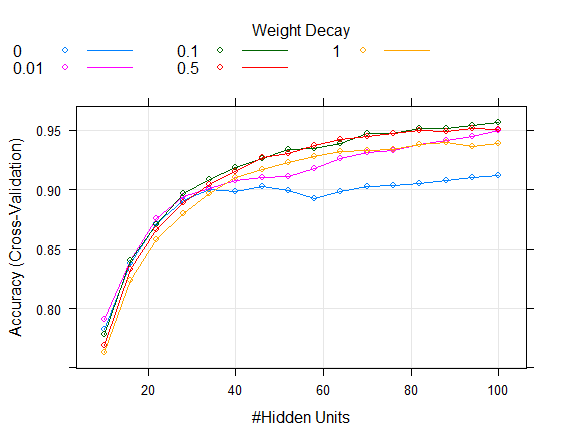
\includegraphics[width=0.8\textwidth]{img/cvMLP.png}
    \caption{Evolució de la predicció de \textit{Cross-Validation}}
    \label{fig:mlpVal}
\end{figure} 

El model aconsegueix un 95.32\% d'encert en el conjunt de dades de prova.

